\chapter{A novel tissue sampling strategy for the elucidation of molecular correlates of visual development}
\textbf{Abstract}\\
\textbf{Throughout visual development, a series of complex connections are established between the retina, lateral geniculate nucleus (LGN), and primary visual cortex (V1).  The extent to which retina, LGN, and V1 substructures may be molecularly distinct from one another has only just begun to be explored.   Here we outline a novel tissue sampling strategy to further characterize molecular influences on the developing visual system, with a specific focus on the development of ocular dominance.  We employ a series of dissection, fluorescent tracing, and optical imaging of intrinsic signal experiments in order to isolate substructures of the retina, LGN, and V1 that provide the anatomical basis of ocular dominance in the ferret.  As an example application of this tissue sampling strategy, isolated tissue is used for proteomic analysis with Two Dimensional Difference Gel Electrophoresis (2D-DIGE).  Briefly, we isolate pairs of fresh tissue samples from temporal and nasal retina, A and A1 LGN layers (corresponding to the contralateral and ipsilateral eyes, respectively), and ipsilateral and contralateral V1 ocular dominance domains for proteomic analysis.  2D-DIGE is used to compare and quantify the protein compliment of these paired tissue samples.  Protein candidates showing differential expression are identified using MALDI-TOF mass spectrometry. Immunohistochemistry and western blot of protein candidates are then used to visualize these differences directly and to characterize their spatiotemporal patterns.}
\pagebreak

\section{Introduction}
In forward looking mammals with overlapping visual fields, segregated eye specific responses to visual stimuli are found in the lateral geniculate nucleus (LGN) and in primary visual cortex (V1).  In the LGN, eye specific projections of retinal ganglion cells (RGCs) are segregated into inputs that range from physiologically distinct projections in the rodents to physiologically and anatomically distinct eye specific laminae in higher mammals.  In the V1, eye specific responses are organized into a salt and pepper distribution of eye specific cells in rodents and into ocular dominance columns in many higher mammals.  The development of these structures in the visual circuit is influenced by both the pattern of neuronal activity in the circuit driven by external stimuli or endogenous activity and patterned gene expression.  
	Hubel and Wiesel$'$s seminal work based on electrode recordings from both normal and visually deprived cats laid the foundation for exploration of the impact of neuronal activity on visual system development.  In the decades since their work,  a large and robust literature has been built up around experimental approaches centered on variations from normal activity as a window on developmental mechanisms.  It has also become clear that there is a strong molecular component to the development of the visual system (Tropea et al., 2009).  
	At the level of the retina, LGN, and V1 there are molecular influences on the structure and function of the visual circuit.  In the retina, RGCs express a suite of known markers that dictate their decussation pattern including transcription factors such as Foxd1 (Herrera et al., 2004), Foxg1 (Tian et al., 2008), Zic2 (Herrera et al., 2003), and Isl2 (Pak et al., 2004) as well as cell surface receptors such as EphB recptors (Williams et al., 2003).  In large part due to these cues, the LGN can be considered to receive nasal retinal input from the contralateral eye and temporal retinal input from the ipsilateral eye.  At the level of the LGN, RGCs express markers that guide their elaboration into appropriate topographic and eye specific target regions such as the Ephrins and Eph receptors which mediate proper retinogeniculate targeting (Flanagan and Vanderhaeghen, 1998; Frisen et al., 1998; Huberman et al., 2005; Pfeiffenberger et al., 2005) and Ten-m3 which affects ipsilateral afferent targeting (Leamey et al., 2007).  In V1, correct topology formation is dependent on EphrinAs and EphAs (Cang et al., 2005) and molecular GABA expression levels shape the width of ocular dominance columns (Hensch, 2005).  
	While we are beginning to understand the impact of many molecular regimes on the developing visual system, it is clear that there is much to learn.  We have a good understanding of the role of only a minority of the full complement of proteins present in the developing visual system.  It is critical that we begin to identify a larger set of proteins at work during visual development in order to diversify and expand our understanding of how patterned gene expression influences visual development.  In order to identify a larger set of proteins involved in visual development, broad based unbiased screening techniques must be employed.  Within the past fifteen years, genetic and proteomic screens have begun to be employed in the study of the developing visual system.  One of the first studies of this kind was demonstrated by Corriveau et al in 1998 when they used differential mRNA display to identify class 1 MHC as a novel player in visual system plasticity (Corriveau et al., 1998).  More recently, a notable study was done by Tropea et al in 2006 using DNA microarrays and RT-PCR in conjunction with  visual deprivation to identify parvalbumin as a novel player in visual system plasticity as well as identifying many other candidates involved in modulating the transduction of inputs to cells in visual cortex (Tropea et al., 2006).  In addition to genetic screens, proteomic based screens have recently been leveraged to study visual development.  Two dimensional difference gel electrophoresis (2D-DIGE) has been used to identify protein candidates that are regulated throughout visual development and are responsive to visual deprivation including synaptotagmin 1 (Cnops et al., 2007a; Cnops et al., 2007c), CRMP2 and CRMP4 (Cnops et al., 2006; Van Den Bergh et al., 2006b; Cnops et al., 2007a; Cnops et al., 2007b).  In addition to comparative studies of age or deprivation condition, 2D-DIGE has been used to characterize the proteome of the visual system relative to other brain areas.  2D-DIGE revealed a list of candidates for areal markers in the cortex including brain type creatine kinase as a novel marker for primary somatosensory cortical (S1) boundaries (Jacobs et al., 2008).  Here, we introduce a methodology for the identification of novel molecular correlates of ocular dominance in the visual system.  We employ a suite of anatomically and functionally guided isolations of ocular dominance substrates in the retina, LGN, and V1 followed by 2D-DIGE and MALDI-TOF mass spectroscopy in order to identify molecular candidates associated with ocular dominance in the developing ferret visual system.

\section{Materials and methods}
\subsection{General animal procedures}
All animal procedures were carried out in accordance with approved protocols for the care and use of animals at Carnegie Mellon University.  For all experiments, animals were deeply anesthetized with either an overdose of sodium pentobarbital delivered through and IP injection (retina and LGN tissue samples) or with 5\% isoflurane in 1:1 O2:N2O (cortical tissue samples) before tissue sample collection. After collection,  all tissue samples were handled in the same manner as described below in Section \ref{DIGE_sample_methods}.

\subsection{Optical imaging of intrinsic signal}
Ferrets ranging in age between P30 and P100 were used for optical imaging of intrinsic signal experiments. Animals were anesthetized and maintained with isoflurane (0.5-1.5\%) and O2:N2O (1:1) for surgical preparation of a cranial imaging window over V1 and V2.   A large craniotomy (5mm) was opened through the skull and the dura resected.  An imaging chamber was constructed over the exposed arachnoid and cortex by interposing a 1\% agarose in 0.9\% sodium chloride saline solution between the brain and a custom coverslip.  This chamber was then secured to the skull using dental cement.  Animals were next paralyzed with pancuronium bromide (0.02mg/kg/hr) and artificially respirated through an endotracheal tube.  Optical imaging of intrinsic signal was carried out using a tandem macroscope lens mounted on a CCD camera (M60; Dalsa, Waterloo, Ontario, Canada) controlled by a commercial data acquisition package (Optical Imaging, Inc., New York, NY 10019) as described previously (Frostig et al., 1990; Bonhoeffer and Grinvald, 1996).  Using this technique, it is possible to track localized cortical metabolic activity in vivo based on changes the optical properties of the tissue.   Briefly, differential reflection of 700nm light off of the exposed V1/V2 cortical surface was recorded in response to visual stimuli generated using a commercial stimulus generator (ViSaGe; Cambridge Research Systems, Rochester, England) presented on a Sony 24�� monitor.  Ocular dominance mapping stimuli consisted of drifting full field square wave grating patterns at a spatial frequency of .125 cycles/degree. Grating patterns were drifted back and forth along the axis orthogonal to the grating orientation at a velocity of 2 cycles/second.  Grating patterns at 0,45,90, and 135 degrees were presented separately to each eye and the differential response between eyes across all patterns presented was taken as the map of ocular dominance.     

\subsection{Retina tissue sampling}
Ferrets ranging in age from P15 to P20 were used for retina sample generation. After injection with sodium pentobarbital, both of the eyes were removed and all further procedures were carried out on ice.  First, the frontal segment and vitreous humor of eye was removed.  The retina was then carefully removed from the retinal pigmented epithelium while leaving it in tact.  The retina was then cut along the ventral to dorsal axis isolating the temporal and nasal portions of the retina from one another.  Samples were pooled between the two retinas for each animal to form single animal temporal and nasal samples for further processing Samples were then homogenized in 30$\mu$l of lysis buffer (7M urea, 4\% CHAPS, 2M thiourea, 10mM DTT) prior to 2D-DIGE.

\subsection{LGN tissue sampling}
Ferrets ranging in age from P15 to P20 were used for LGN tissue sample generation. Two days before LGN tissue sample collection, one eye was injected with cholera toxin $\beta$-subunit conjugated to alexa-488 and the other with cholera toxin $\beta$-subunit conjugated to alexa-555 under isoflurane anesthesia in order to visualize the organization of the retinogeniculate projection.  After injection with sodium pentobarbital, the brain was removed from the skull and the thalamus removed from the brain.  The lateral aspect of the thalamus was sectioned at 300�m using a vibratome.  The alexa labeled LGN laminae were then isolated using under fluorescencently guided micro-dissection as described previously (Kawasaki, 2004)(figure 2.1).  The A and A1 laminae samples were pooled across the two LGNS to form single animal A and A1 samples and homogenized in 30$\mu$l of lysis buffer (7M urea, 4\% CHAPS, 2M thiourea, 10mM DTT) prior to 2D-DIGE.

%------------------------------------LGN sampling fig -----------------------------------------------
\begin{figure}[htb!]
\begin{center}
\leavevmode
\includegraphics[width=1.0\textwidth]{FigureImages/LGNDissection.png}
\end{center}
\caption[Fluorescent micro-dissection of the LGN for 2D-DIGE.]{Fluorescent micro-dissection of the LGN for 2D-DIGE.  A, schematic of the LGN in sagittal section.  Sagittal sections allow for easy visualization and isolation of labeled laminae.  B, intact LGN.  C, LGN with C laminae removed. D, isolation of the A1 lamina. E, the A lamina before separation from the perigeniculate nucleus (PGN) at the ventromedial boundary of the LGN.  F, the A laminae isolated from the rest of the thalamus.  Scale bar = 250�m, applies to all.}
\end{figure}


\subsection{Cortical tissue sampling}
Ocular dominance maps generated using optical imaging of intrinsic signal were segmented into regions of high ocular preference (defined as pixels falling in the first and fourth quartiles of the difference image pixel value distribution).  Segmented ocular dominance maps were used in conjunction of with a green light (546nm) image of cortical surface vasculature to target tissue biopsies of functionally defined ocular dominance columns (Figure 2.2a-d).  Tissue biopsies were taken using one of two approaches.  In the first, fluorescent tracer injections of red and green fluorescent microspheres were used to visualize ocular dominance columns during postmortem dissection of the visual cortex (Figure 2.2e).  In the second approach, a blunted 25 gauge needle (inner diameter = 300$\mu$m) attached to a suction line was lowered into the cortex to a depth of 500$\mu$m.  The needle was then slowly removed from the cortex.  The resulting biopsies were spatially confined to the inner diameter of the needle and minimally disturbed the surrounding tissue.  Biopsies included only cortical grey matter while leaving the underlying white matter in tact, as confirmed by post-mortem inspection of the biopsy site (Figure 2.2f).  Tissue biopsies from 2-3 ocular dominance columns were pooled into two sample tubes according to eye preference.  Samples were then homogenized in 30$\mu$l of lysis buffer (7M urea, 4\% CHAPS, 2M thiourea, 10mM DTT) prior to 2D-DIGE.

%------------------------------------Cortical sampling fig -----------------------------------------------

\pagebreak
\begin{figure}[htb!]
\begin{center}
\leavevmode
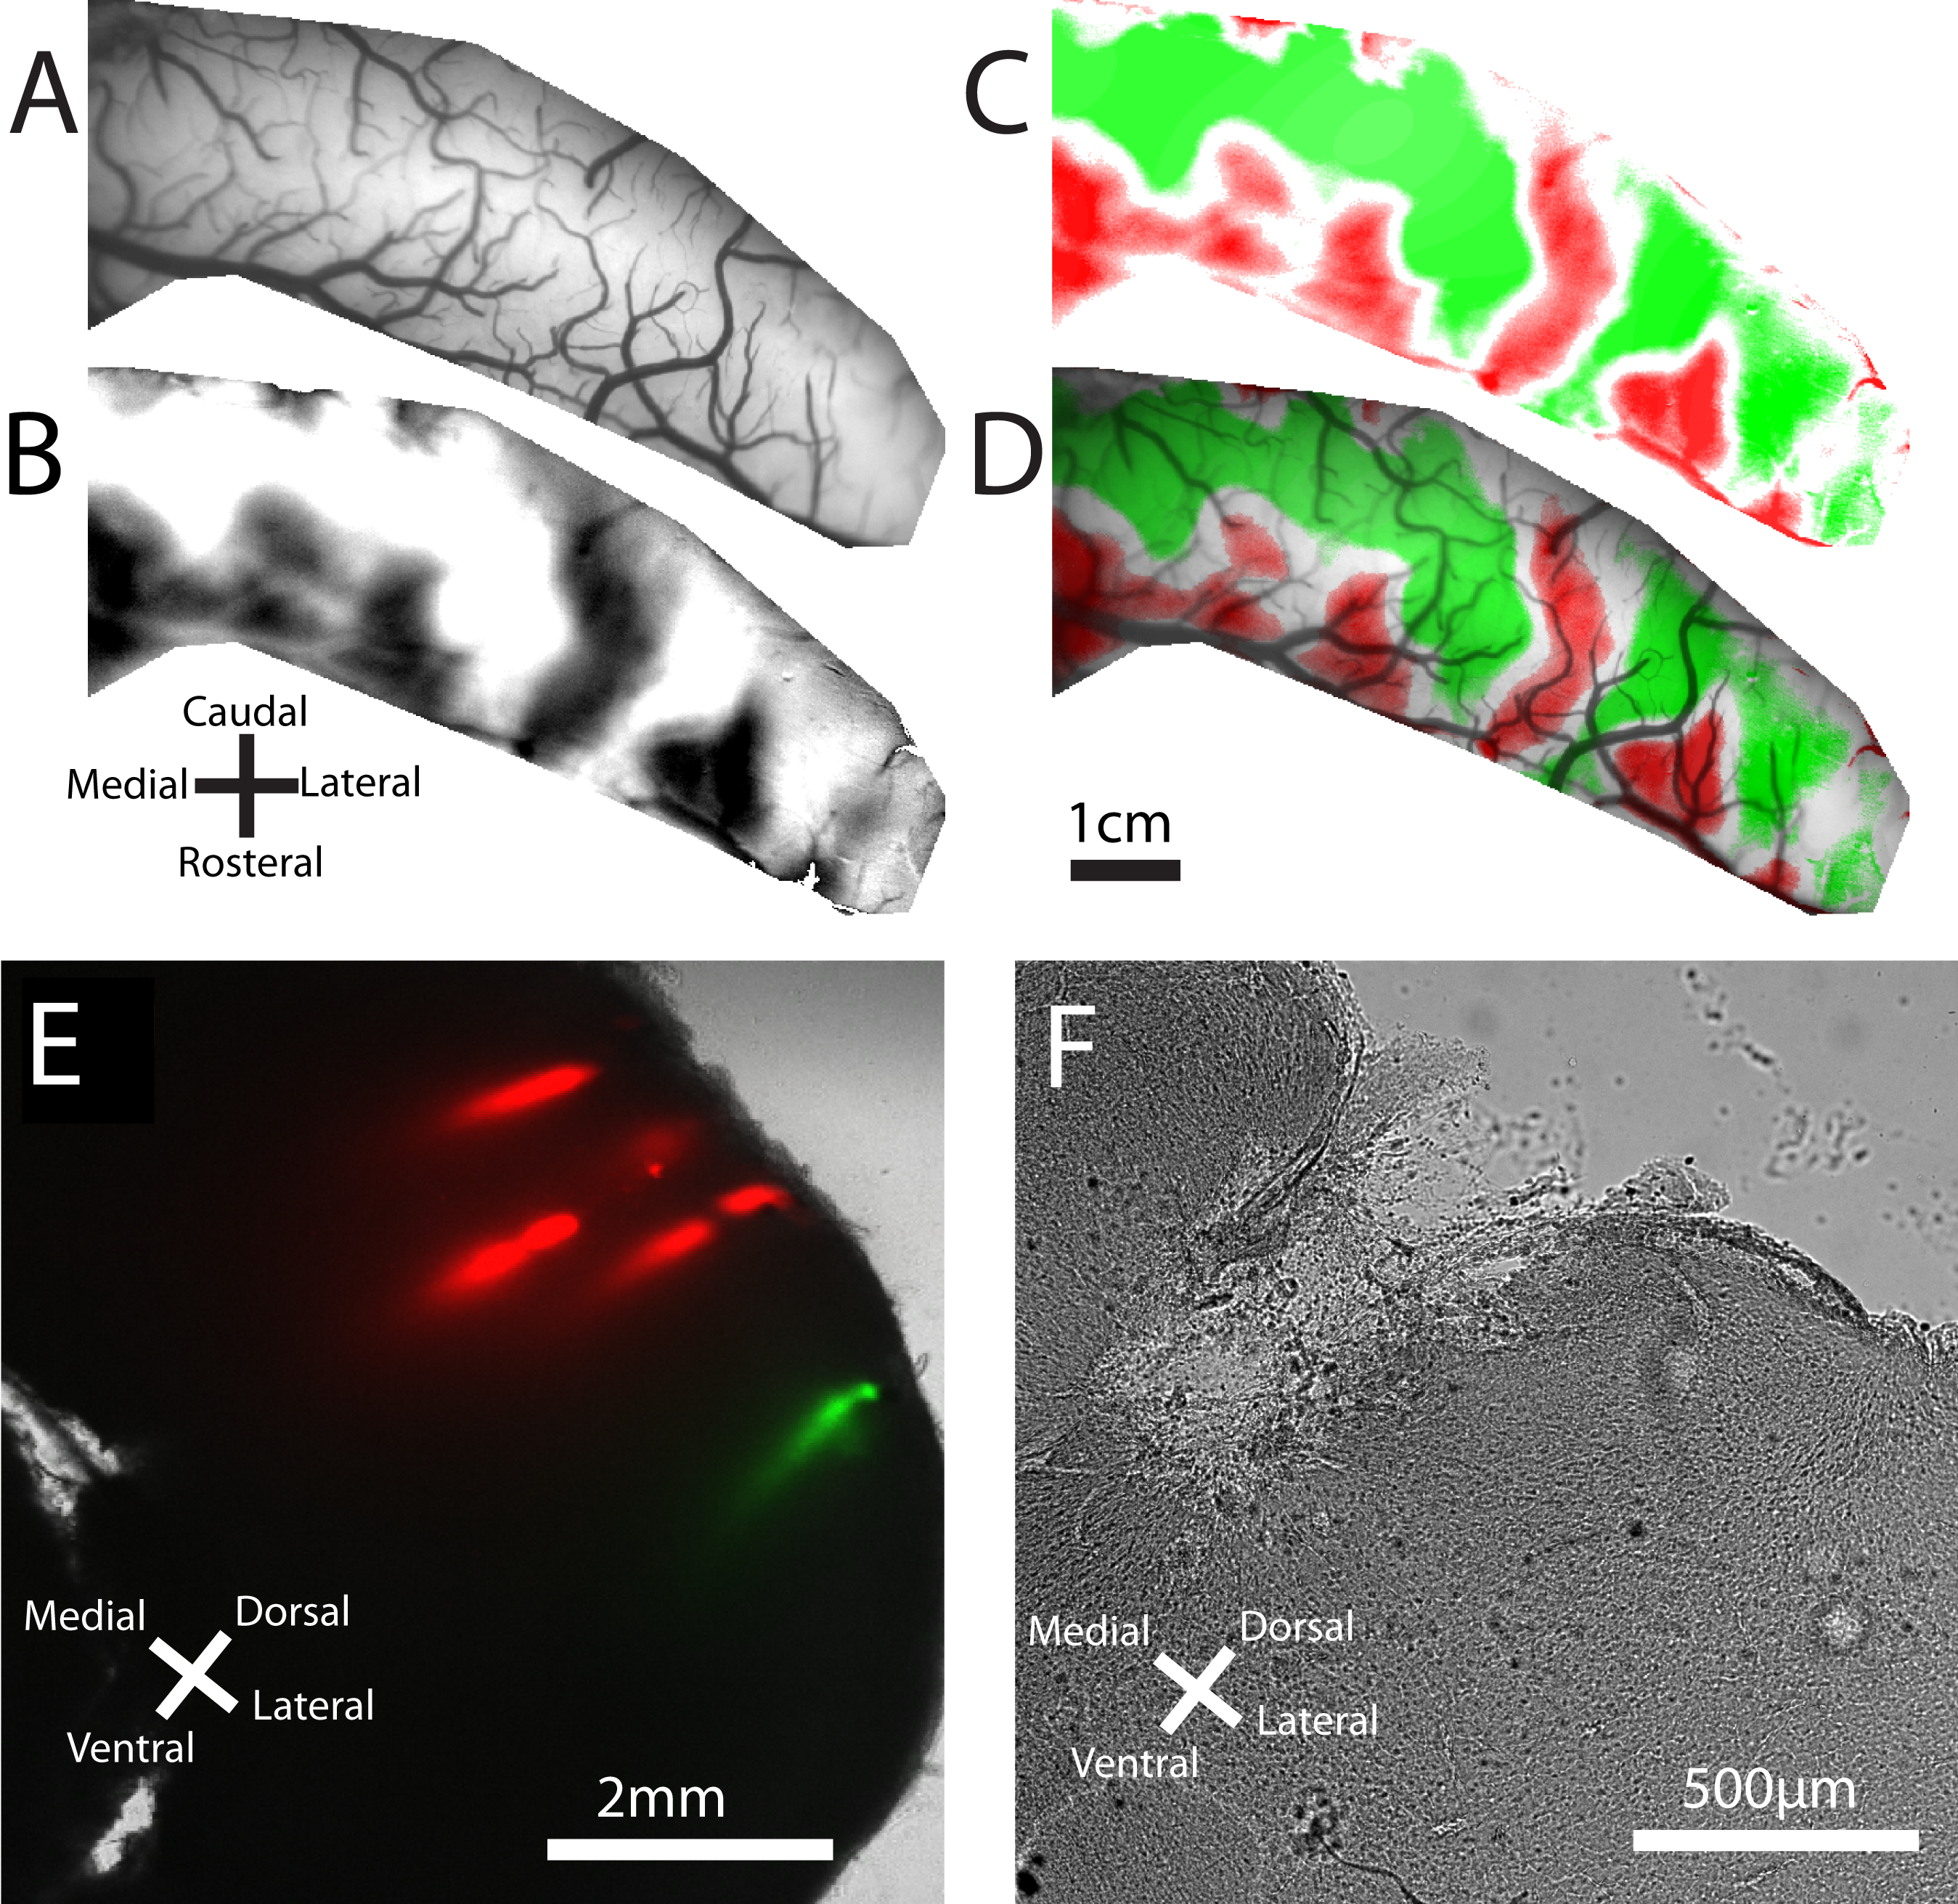
\includegraphics[width=0.8\textwidth]{FigureImages/OItoDIGE.png}
\end{center}
\caption[Isolation 2D-DIGE samples from functionally defined maps of ocular dominance.]{Isolation 2D-DIGE samples from functionally defined maps of ocular dominance.  A, blood vessel map of the dorsal surface of ferret visual cortex illuminated under green light (546nm).  B, functional map of ocular dominance generated using intrinsic signal optical imaging under red light (700nm).  The light patches in B are preferentially responsive to stimuli presented to the contralateral eye, patches in black respond t stimuli presented to the ipsilateral eye.  C,  example map of 2D-DIGE suction biopsy target sites.  Contralateral targets are pseudo-colored in green and ipsilateral targets in red.  D, overlay of biopsy targets onto the blood vessel map from A.  This image is used to visualize the functional map relative to the blood vessel map in order to manually target either fluorescent tracer injections or suction biopsies.  E, postmortem coronal section through a set of tracer injections.  Tracers are used for fluorescence guided micro-dissection of ipsilateral and contralateral responsive domains.  F, postmortem coronal section through a biopsy site.  The biopsy extends ~750�m into the cortex and is ~400�m in diameter.  Biopsies of this size and shape are ideal for specific biopsy of ocular dominance columns in vivo. Blood vessel and functional map courtesy of  D.E. Whitney.}
\end{figure}

\subsection{Two dimensional difference gel electrophoresis}
\label{DIGE_sample_methods}
Sample protein concentration was estimated using a Bradford assay.  The optical density of protein samples was measured at 595nm and compared to a standard curve ranging from .5 mg/ml to 2.5 mg/ml.  Typical sample concentrations were between 1 and 2 mg/ml.  Sample concentrations were then used to balance protein load across sample types for each experiment. Typical experiments yielded approximately 100?g of total protein between the two ocular dominance sample types.  Each sample was minimally labeled with either propyl-Cy3 or methyl-Cy5 dyes (Amersham Biosciences/GE healthcare Piscataway, NJ 08855).  The labeling reaction for these dyes is carried out at sub-stoichiometric conditions, resulting in approximately 5\% of the proteins forming a single bond to a dye molecule.  These dyes are charge and mass matched and run together through 2D-DIGE. The unlabeled portion of the sample runs slightly faster on the gel with a predictable shift, allowing for easy isolation of this protein pool based on the location of the minimally labeled protein pool.  
For labeling, protein samples were made up to 80?l in lysis buffer.  Proteins solutions were minimally labeled with propyl-Cy3 or methyl-Cy5 dyes by incubation with 1?l of the appropriate dye for 15 minutes in the dark and on ice.  Immediately thereafter, non-reacted dye was quenched with an incubation in 1?l of a solution of 5M methylamine-HCl and 10mM HEPES at pH 8.0 for 30 minutes.   The two differentially labeled samples were then mixed together in preparation for co-electrophoresis.  In order to ensure that enough protein was run in our gels for successful identification using mass spectrometry, an unlabeled sample of V1 homogenate was added to the labeled sample mixture.  We have found that increasing the total protein load in our gels using this background sample results in a large increase the number of successfully identified candidate proteins. As an example, only 12\%(3 of 25) spots sampled (see section 2.2.8) from an experiment run without a background were identified and 83\%(10 of 12) samples from an experiment with a background were identified.  The unlabeled V1 homogenate was derived from a mixture of V1 homogenate from a P33 and a P89 normal ferret.  These time points represent the beginning and the end of the critical period in ferret and served as an unbiased background of protein pooled across both development and ocular dominance column type.  
After sample labeling, isoelectric focusing (IEF) was carried out to separate our samples by pH.  IEF was done using a nonlinear immobilized pH gradient strip ( pH 3-10 NL, 13 cm Immobiline DryStips, Amersham Biosciences/GE healthcare) on an IPGphor IEF apparatus (Amersham Biosciences/GE Healthcare), following the manufacturer�s instructions.  IEF was carried out using 500V for 1 hour, 4000V for 1 hour, 8000V for 2 hours, and 8000V until a total of 40kVh was reached.  A typical IEF run took approximately 15 hours to complete using these settings.  After IEF, the immobiline strips were equilibrated for 15 minutes each in two equilibration solutions.  Each equilibration solution contained 50mM Tris, 6M Urea, 30\% glycerol, 2\% SDS, 1\% IPG buffer, and a few grains of bromophenol blue.  Additionally, The first equilibration solution contained 1\% DTT and the second contained 2.5\% iodoacetimide.  After equilibration, the IPG strips were run on a 1mm thick 10-15\% SDS-polyacrylamide gradient gel in the vertical Protean II xi cell (BioRad, Hercules, CA 94547) at 20mA/gel at 4�C. Typical second dimension gel runs lasted between 10 and 12 hours.  After electrophoresis was complete, the final 2D-DIGE gel was fixed in a solution of 40\% HPLC grade methanol and 1\% glacial acetic acid for at least two hours prior to fluorescence imaging for protein spot localization.

\subsection{Fluorescence gel imaging and image analysis}
2D-DIGE gels were imaged using a custom built fluorescent imager in the laboratory of Jonathan Minden of the department of biological sciences at Carnegie Mellon University (Unlu et al., 1997; Viswanathan et al., 2006).  The imager consists of a motorized stage (New England Affiliated Technology, Lawrence, MA 01841) enclosed in a light-tight cabinet fitted with two 250W quartz-tungsten-halogen light sources (Oriel, Irvine, CA 92606) for gel illumination.  For Cy3 or Cy5 specific illumination, light from the light sources is passed through an appropriate band-pass wavelength filter (Chroma Technology, Rockingham, VT 05101 USA) and directed onto the gel via fiber optic light guides (Oriel).  Emission from excited dye molecules is recorded using a cooled 16-bit CCD camera (Photometrics/Roper Scientific, Tucson, AZ 85706) fitted with a 105-mm macro lens (Nikon, Melville, NY 11747-3064, U.S.A.).  By moving the stage relative to the stationary illumination and imaging system under control of custom software, a mosaic image of the entire 20cmx20cm gel is created with a resolution of 135$\mu$m/pixel sufficient for both qualitative and quantitative protein spot identification.  Mosaic gel images were created by exposing all portions of the gel to 30 seconds of illumination at the excitation wavelength of Cy3 followed by 30 seconds of exposure to the excitation wavelength of Cy5.  This exposure time was chosen in order to bring the brightest pixels in the image close to but not above the saturation point of the CDD camera.  Photobleaching was not observed during the imaging sessions.  

Qualitative differences between the Cy3 and Cy5 signals within a gel were appraised using false colored images generated from the raw fluorescence data using ImageJ.  Raw images were log transformed in order to facilitate the visualization of both low and high abundance proteins in the same image.  Next, both images were adjusted for overall brightness to compensate for uneven fluorescence yields between the two dyes.  A red and green overlay image was then constructed from the two adjusted grayscale images.  Protein spots visibly appearing red or green in this overlay image were said to differentially expressed across the samples in the gel.
Quantitative differences between the Cy3 and Cy5 signals were detected using custom software written in MATLAB.  The raw data images were log transformed and additionally median filtered with a 3x3 kernel to remove shot noise.  The centers of all detectable protein spots in the two pre-processed images were found using a custom blob detection algorithm.  Once spot centers were identified, a 9-pixel (1.215mm) diameter region of interest around each center was taken into consideration for further analysis.  For each spot center, the ratio and difference between the Cy3 and Cy5 image was calculated.  From these measurements, a population of ratios and differences was constructed.  Those spot measurements falling two standard deviations above or below the mean difference or ratio were considered to be differentially expressed across the samples in the gel.

\subsection{Protein spot isolation and identification}
Protein spots determined to be differentially expressed between sample types were excised from the 2D-DIGE gel using an automated spot cutter (Applied Precision, Inc, Issaquah, WA 98027) built into the imager used to image the gels.  Protein spots were cut out of the gel under the control of custom software and placed in a 96-well automated protein digester plate (Digilab/Genomic Solutions, Ann Arbor, MI 48108) filled with 1\% glacial acetic acid.  After spot cutting, the wells of the plate were drained of liquid and the excised gel pieces were stored at -80$\degree$C until further processing.  For peptide extraction, gel pieces were thawed and subjected to in-gel tryptic digestion using 20?g of sequencing grade modified trypsin (Promega, Madison, WI 53711 USA) in a ProGest automated protein digester (DigiLab/Genomic Solutions) according to the manufacturer�s instructions.  Peptide extracts were then desalted and concentrated using ZipTip C18 reverse-phase chromatography (Millipore, Billerica, MA 01821).  The tip was rinsed twice in 100\% acetonitrile and twice in .2\% formic acid.  Peptide samples were loaded onto the tip by aspirating the peptide extract through the tip ten times.  The tip was then washed twice in .2\% formic acid and eluted into a sample tube by aspirating ten times with 2.5$\mu$l of a 1:1 100\% ACN:.2\% formic acid solution.
  
Following desalting and concentration, peptide samples were immediately prepared for matrix-assisted laser desorbtion/ionization time of flight (MALDI-TOF) mass spectrometry.  Samples were spotted in a 1:1 ratio with Alpha-Cyano-4- hydroxycinnamic acid matrix (Agilent Technologies, Santa Clara, CA, 95051) on a 100 well stainless steel sample plate (PerSeptive Biosytems/Applied Biosciences, Foster City, Ca, 94404) and allowed to dry.  MALDI-TOF mass spectrometry was then carried out on a Voyager-DE STR mass spectrometer (Applied Biosciences, Foster City, Ca, 94404).  
  
A voltage of 20kV was applied to the sample plate and the matrix was excited with 337nm light from a nitrogen laser.  A peptide survey spectrum was acquired from 750 to 3800 m/z.  A peak list for each spectrum was generated through analysis with Data Explorer (Applied Biosciences, Foster City, Ca, 94404).  Protein identifications were determined by matching sample MALDI-TOF peak lists to the MASCOT MS Fingerprint database (Perkins et al., 1999).  MASCOT searches were carried out with a fixed modification of carboxymethl, variable modification of methionine oxidation, one possible missed trypsin cleavage, and within a range of 50ppm.

\subsection{Immunohistochemistry}
All immunohistochemical stains were carried out using primary antibodies at a dilution of 1:500 (CRMP4, cat. \#AB5454, Millipore, Billerica, MA; munc13-3, cat. \#ab2707 Abcam, Cambridge, MA; CRMP2, gift from Dr. Rajesh Khanna, Indiana University).  For munc13-3 and CRMP4 stains, expression was assayed with a primary antibody followed by a fluorescent secondary antibody (Alexa 594 or Alexa 488, 1:500 dilution, Invitrogen, Carlsbad, CA).  For CRMP2 stains, a biotinylated secondary antibody (cat. \#BA-1000, Vector Laboratories, Burlingame, CA) was detected using the Vectastain Elite ABC kit (cat. \#PK-6101, Vector Laboratories, Burlingame, CA).

\section{Results}
\subsection{Retinal molecular correlates of visual development}
Three 2D-DIGE experiments were conducted on retinal tissue derived from temporal and nasal tissue as described in 2.2.3.  From these three experiments, eleven protein candidates were found to be differentially expressed.  No protein candidate was found in more than one experiment.  Four of the candidates were expressed in the temporal retina and seven were expressed in the nasal retina (table 2.1).  The isolated proteins were localized primarily in the cytoplasm (6, 54.55\%) , with a minority of the proteins in the set localized to the cytoskeleton (2, 18.18\%), nucleus (2, 18.18\%), and the plasma membrane (1, 9.09\%) (figure 2.3).  The functional roles of protein candidates were dominantly structural in nature(4, 36.36\%).  Minority fractions of the candidates were involved in chaperone (2, 18.18\%), enzyme (2, 18.18\%), splicing (1, 9.09\%), metabolic (1, 9.09\%), and neurotransmitter release (1, 9.09\%) functions (figure 2.4).  

From the list of protein candidates differentially expressed between the temporal and nasal retina, munc13-3 was chosen for further validation by immunohistochemistry.  In  one 2D-DIGE experiment, munc13-3 was found to be expressed in higher abundance in the temporal portion of the retina.  The munc13 family regulates synaptic transmission by catalyzing  the partial formation of  SNARE complexes required for neurotransmitter release (Pang and Sudhof, 2010).  Munc13 proteins are known regulators of ribbon synapses in retinal photoreceptors and are therefore of potential importance in the formation and maintenance of retinothalamic projections (tom Dieck et al., 2005).   Munc13-3 is primarily expressed in non-cortical neural tissues and is hypothesized to work in concert with munc13-1 to regulate synaptic transmission in these tissues (Augustin et al., 1999).  Immunohistochemistry against munc13-3 in two flat mounted ferret retinas aged P17 and P25 show a trend of relative over expression of munc13-3 in the temporal aspect of the retina (figure 2.5).  To further characterize the expression of munc13-3 in the developing retina, immunohistochemistry against munc13-3 in was carried out in horizontal sections of P13 retinas.  Munc13-3 appeared to stain puncta in the retinal ganglion cell layer of both the temporal and nasal portions of the retina.  Stained puncta were more dense in the temporal retina than in the nasal retina (figure 2.6).  This result taken with the observed temporal bias in expression from P17 and P25 flat mounted retinas do not definitively confirm the temporal bias in expression found in the temporal/nasal 2D-DIGE screen, but lend support to it.


%------------------------------------Begin Retina Figures -----------------------------------------------

\pagebreak
\begin{figure}[htb!]
\begin{center}
\leavevmode
\includegraphics[width=1.0\textwidth]{FigureImages/RetCandidateLocations.png}
\end{center}
\caption[Location of protein candidates found to be differentially expressed across temporal and nasal retina.]{Location of protein candidates found to be differentially expressed across temporal and nasal retina.  Eleven protein candidates were found to be differentially expressed across the temporal and nasal retina. The number of candidates found in each sub-cellular location is displayed inside of each pie slice. The majority of protein candidates are were localized to the cytoplasm (6, 54.55\%) with a minority found in the cytoskeleton (2, 18.18\%), nucleus (2, 18.18\%), and the plasma membrane (1, 9.09\%).}
\end{figure}

\pagebreak
\begin{figure}[htb!]
\begin{center}
\leavevmode
\includegraphics[width=1.0\textwidth]{FigureImages/RetCandidateFunctions.png}
\end{center}
\caption[Functions of protein candidates found to be differentially expressed across temporal and nasal retina.]{Functions of protein candidates found to be differentially expressed across temporal and nasal retina.  Eleven protein candidates were found to be differentially expressed across the temporal and nasal retina. The number of candidates found in each functional category is displayed inside of each pie slice. The majority of protein candidates are structural in nature(4, 36.36\%).  Minority fractions of the candidates are involved in chaperone (2, 18.18\%), enzyme (2, 18.18\%), splicing (1, 9.09\%), metabolic (1, 9.09\%), and neurotransmitter release (1, 9.09\%) functions.}
\end{figure}

\pagebreak
\begin{figure}[htb]
\begin{center}
\leavevmode
\includegraphics[width=1.0\textwidth]{FigureImages/munc13_flat_retina_quant.png}
\end{center}
\caption[Quantification of munc13-3 expression in the flat mounted retina.]{Quantification of munc13-3 expression in the flat mounted retina.  A, flat mount view of a P17 retina stained for munc13-3.  There is a trend of higher expression on in the temporal leaflet when compared to the nasal leaflet.  B, The same image smoothed and then binned into 20�m domains for quantification.  The domains over the center of the retina (black box in B) were used to compute nasal to temporal linescans shown in C.  The location of the optic nerve head is shown by the gray line in B and C. C, each nasal to temporal linescan is shown in blue with the average linescan shown in black.   There is higher munc13-3 expression on the nasal portion of the retina as defined by the location of the optic nerve head.  D, high magnification view of munc13-3 expression in the nasal leaflet of a P17 retina.  E, high magnification view of munc13-3 expression in the temporal leaflet of a P17 retina.  When normalized to the total number of cells in the field of view, 25\% of the nasal cells and 29\% of the temporal cells express munc13-3.  Scale bar=50�m and applies to both D and E.}
\end{figure}  

\pagebreak
\begin{figure}[htb]
\begin{center}
\leavevmode
\includegraphics[width=1.0\textwidth]{FigureImages/munc13-3_horiz.png}
\end{center}
\caption[Munc13-3 expression in retinal cross-sections.]{Munc13-3 expression in retinal cross-sections.  A, no primary control in a section through a P13 retina.  There is observable autofluorescence in all layers of the retina.  B and C, munc13-3 stain in the temporal and nasal portions of the same retina.  There is specific expression above the baseline autofluorescence of munc13-3 in both the nasal and temporal retina.  D and E, enlarged view of the boxes in D and C with the locations of munc13-3 positive puncta overlaid by red dots.  F, the density of munc13-3 positive puncta is higher in the nasal retina than in the temporal retina.}
\end{figure}
%------------------------------------ End Retina Figures -----------------------------------------------

%------------------------------------ Begin Retina Tables -----------------------------------------------
\doublespacing 
\pagebreak
\definecolor{lightgray}{rgb}{0.8,0.8,0.8}
\rowcolors{2}{lightgray}{white}
\begin{center}\scriptsize
\begin{longtable}{m{2cM} m{1.5cM} m{1cM} m{1.2cM} m{2cM} m{.8cM} m{0.5cM} m{0.6cM} m{1cM}}
\caption[List of protein candidates found to be differentially expressed across temporal and nasal retina.]{List of protein candidates found to be differentially expressed across temporal and nasal retina.}\\
\hline
{\bf Protein Name} & {\bf Expression Direction} & {\bf Total Hits} & {\bf EI \newline(T-N) /(T+N)} & {\bf Matched Species} & {\bf MW\newline(Da)} & {\bf pH} & {\bf Score} & {\bf Coverage} \\ 
\hline
\endfirsthead
\endhead
\hline
{{Continued on next page}} \\ 
\hline
\endfoot
\hline \hline
\caption*{Protein candidates are listed alphabetically.  EI: expression index defined as (Temporal expression - Nasal Expression)/(Temporal expression + Nasal Expression).  Matched Species: identity of the species to which the MS data was matched.  MW: predicted molecular weight in daltons.  pH: predicted pH.  Score: MASCOT score.  Coverage: percent of sequence covered by the MASCOT match.}
\endlastfoot
14-3-3 epsilon & Temporal & 1 & 1 & Mus musculus   & 20115 & 4.51 &	100	& 57\\
    alpha tubulin  & Temporal & 1 & 1 & Macaca Mulatta	 & 43315	& 4.94 & 165	& 55\\
    beta A1 crystallin	&Nasal	&1	&-1	&Cavia porcellus	&23668	&6.38	&138 &	61\\
	beta B1 crystallin	&Nasal	&1	&-1	&Bos taurus	&28354	&7.66	&172	 &48\\
	dnaK-type molecular chaperone hsp72	&Temporal	&1	&1	&Rattus norvegicus	&71112	&5.43	&170 &	34\\
	guanine nucleotide-binding protein, beta-1 subunit	&Nasal	&1	&-1	&Canis familiaris	&38151	&5.6 &	76	&36\\
	heat shock 70kDa protein 8	&Nasal	&1	&-1	&Homo sapiens	&53580	&5.62	&230&	44\\
	Heterogeneous nuclear ribonucleoprotein F (hnRNP F)	&Nasal	&1	&-1	&Canis familiaris	&45942	&5.32	&72	&31\\
	Hexokinase, type I (HK I)	&Nasal	&1	&-1	&Canis familiaris	&120076	&8.88	&81	&15\\
	munc13-3	&Temporal	&1	&1	&Macaca Mulatta	&254083	&5.76	&73	&10\\
	protein phosphatase 1, catalytic subunit	&Nasal	&1	&-1	&Homo sapiens	&37945	&5.84	&79	&33\\
\end{longtable}
\end{center}

\begin{center}\scriptsize
\begin{longtable}{m{6cM} m{4cM} m{4cM}}
\caption[List of retinal protein candidates sub-cellular locations and functions.]{List of retinal protein candidates sub-cellular locations and functions}\\
\hline
{\bf Protein Name} & {\bf Protein Location} & {\bf Protein Function} \\ 
\hline
\endfirsthead
\endhead
\hline
{{Continued on next page}} \\ 
\hline
\endfoot
\hline \hline
\caption*{Protein candidates are listed alphabetically. All sub-cellular location and function category assignments are based off of protein candidate entries in the Uniprot online database (Jain et al., 2009).}
\endlastfoot
14-3-3 epsilon										&cytoplasm				&Structural\\
alpha tubulin										&cytoskeleton			&Structural\\
beta A1 crystallin									&plasma membrane			&Structural\\
beta B1 crystallin									&cytoplasm				&Structural\\
dnaK-type molecular chaperone hsp72					&cytoplasm				&Chaperones\\
guanine nucleotide-binding protein, beta-1 subunit		&cytoskeleton			&Enzymes\\
heat shock 70kDa protein 8							&cytoplasm				&Chaperones\\
Heterogeneous nuclear ribonucleoprotein F (hnRNP F)	&cytoplasm				&Splicing Factors\\
Hexokinase, type I (HK I)								&cytoplasm				&Metabolic\\
munc13-3												&nucleus					&Neurotransmitter Secretion\\
Protein phosphatase 1, catalytic subunit				&nucleus					&Enzymes\\
\end{longtable}
\end{center}
\singlespacing
%------------------------------------ End Retina Tables -----------------------------------------------

\subsection{LGN molecular correlates of visual development}
A Total of fourteen differentially expressed protein candidates were identified in four 2D-DIGE experiments on A and A1 LGN laminae as described in 2.2.4.  Three of the candidates were identified in two different experiments, the rest were only identified once. Seven of the candidates were expressed in the A lamina, six were expressed in the A1 lamina, and one candidate was found to be expressed once in the A lamina and once in the A1 lamina (table 2.2).  LGN protein candidates displayed a similar sub cellular pattern to that the observed pattern in retinal 2D-DIGE experiments (2.3.1).  The majority of protein candidates are were localized to the cytoplasm (8, 57.14\%) with a minority found in the cytoskeleton (3, 21.43\%), nucleus (1, 7.14\%), mitochondria (1, 7.14\%), and the endoplasmic reticulum (1, 7.14\%) (figure 2.7).  The functional properties of LGN protein candidates were again dominantly structural in nature(5, 35.71\%).  Minority fractions of the candidates were involved in chaperone (2, 14.29\%), enzyme (1, 7.14\%), metabolic (2, 14.29\%), axon guidance (3, 21.43\%), and proteolytic (1, 7.14\%) functions (figure 2.8).

From the list of identified LGN candidates, collapsin response mediator protein 4 (CRMP4) was chosen for further analysis.  CRMP4 was identified in one 2D-DIGE experiment and was found to be relatively over expressed in the A lamina of the LGN.  CRMP family members have been implicated in growth cone dynamics and guidance and are differentially expressed across the central nervous system (Wang and Strittmatter, 1996).� CRMP2, CRMP4, and CRMP5 show developmentally regulated expression profiles in cat primary visual cortex, indicating a possible role for the CRMP family in visual system patterning (Cnops et al., 2004; Cnops et al., 2006; Van Den Bergh et al., 2006b).� Consistent with a putative role in neural patterning, juvenile CRMP4 expression is high and adult expression is low (Cnops et al., 2004; Cnops et al., 2006; Van Den Bergh et al., 2006b).  Immunostaining against CRMP4 in a P30 LGN demonstrated that CRMP4 was more highly expressed in both the cell sparse interlaminar zones and ON/OFF sub-laminar boundaries than the main lamina (A, A1, C) of the nucleus (see chapter 3, fig 3.1).  The observed CRMP4 expression pattern was found to be developmentally regulated and is characterized in chapter 3.  Further, the expression of CRMP4 in the LGN was found to be sensitive to the local arrangement of the cytoarchitecture in the nucleus.  This result is reported in chapter 4.  The organization of CRMP4 expression in the LGN does not confirm CRMP4 as a marker for the A lamina of the LGN.  The observed CRMP4 expression pattern indicates that the appearance of CRMP4 as an A lamina candidate likely resulted from a sampling error in the micro-dissection of LGN laminae during sample generation.

%------------------------------------Begin LGN Figures -----------------------------------------------

\pagebreak
\begin{figure}[htb!]
\begin{center}
\leavevmode
\includegraphics[width=1.0\textwidth]{FigureImages/LGNCandidateLocations.png}
\end{center}
\caption[List of protein candidates found to be differentially expressed across the A and A1 LGN laminae.]{List of protein candidates found to be differentially expressed across the A and A1 LGN laminae.  Fourteen protein candidates were found to be differentially expressed across the A and A1 LGN laminae. The number of candidates found in each sub-cellular location is displayed inside of each pie slice. The majority of protein candidates are were localized to the cytoplasm (8, 57.14\%) with a minority found in the cytoskeleton (3, 21.43\%), nucleus (1, 7.14\%), mitochondria (1, 7.14\%), and the endoplasmic reticulum (1, 7.14\%).}
\end{figure}

\pagebreak
\begin{figure}[htb!]
\begin{center}
\leavevmode
\includegraphics[width=1.0\textwidth]{FigureImages/LGNCandidateFunctions.png}
\end{center}
\caption[Functions of protein candidates found to be differentially expressed across the A and A1 LGN laminae.]{Functions of protein candidates found to be differentially expressed across the A and A1 LGN laminae.  Fourteen protein candidates were found to be differentially expressed across the A and A1 LGN laminae. The number of candidates found in each functional category is displayed inside of each pie slice. The majority of protein candidates are structural in nature(5, 35.71\%).  Minority fractions of the candidates are involved in chaperone (2, 14.29\%), enzyme (1, 7.14\%), metabolic (2, 14.29\%), axon guidance (3, 21.43\%), and proteolysis (1, 7.14\%) functions.}
\end{figure}

%------------------------------------End LGN Figures -----------------------------------------------
%------------------------------------ Begin LGN Tables -----------------------------------------------
\doublespacing
\pagebreak
\definecolor{lightgray}{rgb}{0.8,0.8,0.8}
\rowcolors{2}{lightgray}{white}
\begin{center}\scriptsize
\begin{longtable}{m{2cM} m{1.5cM} m{1cM} m{1.2cM} m{2cM} m{.8cM} m{0.5cM} m{0.6cM} m{1cM}}
\caption[List of protein candidates found to be differentially expressed across the A and A1 LGN laminae.]{List of protein candidates found to be differentially expressed across the A and A1 LGN laminae.}\\
\hline
{\bf Protein Name} & {\bf Expression Direction} & {\bf Total Hits} & {\bf EI \newline(A1-A) /(A1+A)} & {\bf Matched Species} & {\bf MW\newline(Da)} & {\bf pH} & {\bf Score} & {\bf Coverage} \\ 
\hline
\endfirsthead
\endhead
\hline
{{Continued on next page}} \\ 
\hline
\endfoot
\hline \hline
\caption*{Protein candidates are ordered by highest number of repeat hits from top to bottom.  EI: expression index defined as (A1 expression - A Expression)/(A1 expression + A Expression).  Matched Species: identity of the species to which the MS data was matched.  MW: predicted molecular weight in daltons.  pH: predicted pH.  Score: MASCOT score.  Coverage: percent of sequence covered by the MASCOT match.}
\endlastfoot
collapsin response mediator protein 2	&None	&2	&0	&Canis Familiaris	&74229	&5.98	&172   &	70\\
Chain A, Crystal Structure Of Bovine Hsc70(Aa1-554)e213aD214A MUTANT	&A1	&2	&1	&Bos taurus	&60977	&6.05	&159   &	59\\
alpha tubulin	&A1	&2	&1	&Macaca mulatta	&46781	&4.96	&101	 &56\\
aconitase 2, mitochondrial isoform 3	&A	&1	&-1	&Canis Familiaris	&86409	&8.07	&201   &	36\\
collapsin response mediator protein 1	&A	&1	&-1	&Canis Familiaris	&74485	&6.67	&126	   &48\\
collapsin response mediator protein 4	&A	&1	&-1	&Bos taurus	&74398	&5.98	&72	&42\\
GDP dissociation inhibitor 1 (predicted)	&A1	&1	&1	&Rhinolophus ferrumequinum
	&51060	&4.96	&77	&36\\
beta actin	&A1	&1	&1	&Mus musculus	&39446	&5.78	&94	&35\\
Creatine kinase B-type (Creatine kinase B chain) (B-CK) isoform 1 	&A	&1	&-1	&Equus caballus
	&42976	&5.47	&79	&60\\
ubiquitin carboxyl-terminal esterase L1	&A	&1	&-1	&Sus scrofa
	&25186	&5.22	&101 	&64\\
dystonin isoform 1 isoform 17	&A	&1	&-1	&Canis Familiaris	&632401	&5.51	&71	&17\\
Heat-Shock Cognate 70kd Protein
	&A1	&1	&1	&Bos taurus	&42557	&7.03	&91	&71\\
beta tubulin	&A1	&1	&1	&Homo sapiens	&50274	&4.78	&299    &49\\
keratin 1	&A	&1	&-1	&Homo sapiens	&66149	&8.16	&70	&19\\
\end{longtable}
\end{center}

\pagebreak

\begin{center}\scriptsize
\begin{longtable}{m{6cM} m{4cM} m{4cM}}
\caption[List of LGN protein candidates sub-cellular locations and functions.]{List of LGN protein candidates sub-cellular locations and functions}\\
\hline
{\bf Protein Name} & {\bf Protein Location} & {\bf Protein Function} \\ 
\hline
\endfirsthead
\endhead
\hline
{{Continued on next page}} \\ 
\hline
\endfoot
\hline \hline
\caption*{Protein candidates are listed alphabetically. All sub-cellular location and function category assignments are based off of protein candidate entries in the UniProt online database (Jain et al., 2009).}
\endlastfoot
aconitase 2, mitochondrial isoform 3									&mitochondria			&Metabolic\\
alpha tubulin														&cytoskeleton			&Structural\\
beta actin															&cytoskeleton			&Structural\\
beta tubulin															&cytoskeleton			&Structural\\
Chain A, Crystal Structure Of Bovine Hsc70(Aa1-554)e213aD214A MUTANT	&nucleus					&Chaperones\\
collapsin response mediator protein 1									&cytoplasm				&Axon Guidance\\
collapsin response mediator protein 2									&cytoplasm	 			&Axon Guidance\\
collapsin response mediator protein 4									&cytoplasm				&Axon Guidance\\
Creatine kinase B-type (Creatine kinase B chain) (B-CK) isoform 1 		&cytoplasm				&Metabolic\\
dystonin isoform 1 isoform 17											&cytoplasm				&Structural\\
GDP dissociation inhibitor 1 (predicted)								&endoplasmic reticulum	&Enzymes\\
Heat-Shock Cognate 70kd Protein										&cytoplasm				&Chaperones\\
keratin 1															&cytoplasm				&Structural\\
ubiquitin carboxyl-terminal esterase L1								&cytoplasm				&Proteolysis\\
\end{longtable}
\end{center}
\singlespacing
%------------------------------------ End LGN Tables -----------------------------------------------

\subsection{Cortical molecular correlates of visual development}
Forty-two differentially expressed protein candidates were identified in eleven 2D-DIGE experiments on contralateral and ipsilateral ocular dominance columns as described in 2.2.5.  One of the candidates was identified in four different experiments, four were identified in three different experiments, and four were identified in two different experiments.  All other candidates were only identified once. Twenty-two of the candidates were expressed in contralateral ocular dominance columns, eighteen were expressed in ipsilateral ocular dominance columns, and two candidates were found to be expressed evenly across ocular dominance column types (table 2.3).   As with the retina and LGN  candidates described 2.3.1 and 2.3.2, the majority of cortical protein candidates were localized to the cytoplasm (24, 57.14\%) with a minority found in the cytoskeleton (4, 9.52\%), nucleus (4, 9.52\%), mitochondria (8, 19.04\%), endoplasmic reticulum (1, 2.38\%), and plasma membrane (1, 2.38\%) (figure 2.10).  The breakdown of cortical candidate functional properties showed more candidates involved in enzymatic processes (11, 26.19\%) than candidates from retina and LGN experiments. Minority fractions of the candidates were involved in structural (10, 23.81\%), metabolic (8, 19.05\%), chaperone (5, 11.94\%), axon guidance (2,4.76\%), and proteolysis (1, 2.38\%), or other (5, 11.94\%) functions (figure 2.11).

Collapsin response mediator protein 2 (CRMP2) was chosen for further analysis by immunohistochemistry and western blot.  CRMP2 was identified in two 2D-DIGE experiments and was found to be more highly expressed in ipsilateral ocular dominance columns than in contralateral dominance columns.  As described in 2.3.2, the CRMP family is implicated in axon dynamics and is potentially involved in visual system development.  Western blot against CRMP2 in two animals (P36 and P270) showed a higher level of expression in ipsilateral ocular dominance column samples than in contralateral ocular dominance columns samples, indicating that there the relative expression of CRMP2 may be biased toward ipsilateral columns throughout visual development (figure 2.12).

Immunohistochemical stains against CRMP2 in P12 and P16 animals identified an early phase of CRMP2 expression (figure 2.13, A and B) in which discrete patches of CRMP2 expression are visible in the the neuropil of the visual cortex.  These CRMP2 patches are variable in their size and spacing and are not evenly distributed across the cortex as would be expected of a pattern mirroring the distribution of ocular dominance columns (figure 2.13, C). Animals in the early visual critical period  do not appear to CRMP2 expression in immunohistochemical stains.  At the end of the visual critical period,  the expression of of CRMP2 is only apparent toward near the V1/V2 border.  At this age and into adulthood, CRMP2 expression is limited to a discrete band of cells across the cortex near the V1/V2 border.  In the ferret, it has been observed that there is a large band of V2 cells responsive to ipsilateral inputs at the V1/V2 border (White et al., 1999b).  The location of the CRMP2 positive band of cells appears to localize well with this large ipsilateral response domain (figure 2.14).  These experiments along with the finding that CRMP2 is expressed in the A1 lamina of the LGN in a 2D-DIGE experiment lend support to the hypothesis that CRMP2 may be involved in visual development and/or maintenance in the ferret. Specifically, CRMP2 may be involved in the maintenance of the V1/V2 border in early development and adulthood.

%------------------------------------Begin Cortical Figures -----------------------------------------------

\pagebreak
\begin{figure}[htb!]
\begin{center}
\leavevmode
\includegraphics[width=1.0\textwidth]{FigureImages/CorticalCandidateLocations.png}
\end{center}
\caption[Location of protein candidates found to be differentially expressed across contralateral and ipsilateral ocular dominance columns.]{Location of protein candidates found to be differentially expressed across contralateral and ipsilateral ocular dominance columns.  Forty-two protein candidates were found to be differentially expressed across contralateral and ipsilateral ocular dominance columns. The number of candidates found in each sub-cellular location is displayed inside of each pie slice. The majority of protein candidates are were localized to the cytoplasm (24, 57.14\%) with a minority found in the cytoskeleton (4, 9.52\%), nucleus (4, 9.52\%), mitochondria (8, 19.04\%), endoplasmic reticulum (1, 2.38\%), and the plasma membrane (1, 2.38\%).}
\end{figure}

\pagebreak
\begin{figure}[htb!]
\begin{center}
\leavevmode
\includegraphics[width=1.0\textwidth]{FigureImages/CorticalCandidateFunctions.png}
\end{center}
\caption[Functions of protein candidates found to be differentially expressed across contralateral and ipsilateral ocular dominance columns.]{Functions of protein candidates found to be differentially expressed across contralateral and ipsilateral ocular dominance columns.  Forty-two protein candidates were found to be differentially expressed across contralateral and ipsilateral ocular dominance columns. The number of candidates found in each functional category is displayed inside of each pie slice. The majority of protein candidates were enzymes (11, 26.19\%).  Minority fractions of the candidates were involved in structural (10, 23.81\%), metabolic (8, 19.05\%), chaperone (5, 11.94\%), axon guidance (2,4.76\%), and proteolysis (1, 2.38\%), or other (5, 11.94\%) functions.}
\end{figure}

\pagebreak
\begin{figure}[htb!]
\begin{center}
\leavevmode
\includegraphics[width=0.7\textwidth]{FigureImages/CRMP2_Western.png}
\end{center}
\caption[Western blot of ipsilateral and contralateral ocular dominance column CRMP2 expression]{Western blot of ipsilateral and contralateral ocular dominance column CRMP2 expression.  Western blot reveals a relative abundance of CRMP2 expression in ipsilateral ocular dominance column samples relative to contralateral ocular dominance column samples.  Glyceraldehyde 3-phosphate dehydrogenase (GAPDH), a ubiquitous metabolic protein found in the brain is used as a control.  CRMP2 bands run at ~60 kDa in good agreement with the known mass of human CRMP2 at 62,294 Da.}
\end{figure}

\pagebreak
\begin{figure}[htb!]
\begin{center}
\leavevmode
\includegraphics[width=1.0\textwidth]{FigureImages/CRMP2Timecourse.png}
\end{center}
\caption[Time-course of CRMP2 expression in the visual cortex]{Time-course of CRMP2 expression in the visual cortex.  Immunohistochemical staining against CRMP2 reveals an early phase of CRMP2 expression (P12 and P16, A and B) that is localized to discrete patches in the neuropil. CRMP2 patches have variable size and spacing making it unlikely that they are marking ocular dominance columns.  Animals in the early critical period do not show robust CRMP2 expression (P31, C).  Toward the end of the critical period and into adulthood, animals begin to show expression of CRMP2 in a small band of cells across the medial to lateral extent of the the visual cortex.  Scale bars = 200$\mu$m.}
\end{figure}

\pagebreak
\begin{figure}[htb!]
\begin{center}
\leavevmode
\includegraphics[width=0.75\textwidth]{FigureImages/CRMP2Overlay.png}
\end{center}
\caption[CRMP2 is expressed near the V1/V2 border in the mature visual cortex]{CRMP2 is expressed near the V1/V2 border in the mature visual cortex.  A, coronal section through a P106 ferret cortex stained for CRMP2.  Positively expressing cells appear as a dark stain.  A thin band of cells express CRMP2 across the medial to lateral extent of the cortex.  B, higher magnification view of the box in A.  C, dorsal view of a reconstruction of sequential coronal sections through the cortex.  Areas that are positive for CRMP2 expression appear as black patches.  D, Ocular dominance map from the same animal.  E, overlay of the slice reconstruction series on the functional map in D.  The overlay was warped based on marker injections made into the cortex and reconstructed post mortem (not shown).  The red asterisk in C and E denotes the position of the slice shown in A and B in the coronal series.  Scale bars = 200$\mu$m.}
\end{figure}

%------------------------------------End Cortical Figures -----------------------------------------------
%------------------------------------ Begin LGN Tables -----------------------------------------------
\doublespacing
\pagebreak
\definecolor{lightgray}{rgb}{0.8,0.8,0.8}
\rowcolors{2}{lightgray}{white}
\begin{center}\scriptsize
\begin{longtable}{m{2cM} m{1.5cM} m{1cM} m{1.2cM} m{2cM} m{.8cM} m{0.5cM} m{0.6cM} m{1cM}}
\caption[List of protein candidates found to be differentially expressed across ipsilateral and contralateral ocular dominance columns]{List of protein candidates found to be differentially expressed across ipsilateral and contralateral ocular dominance columns}\\
\hline
{\bf Protein Name} & {\bf Expression Direction} & {\bf Total Hits} & {\bf EI \newline(I-C) /(I+C)} & {\bf Matched Species} & {\bf MW\newline(Da)} & {\bf pH} & {\bf Score} & {\bf Coverage} \\ 
\hline
\endfirsthead
\endhead
\hline
{{Continued on next page}} \\ 
\hline
\endfoot
\hline \hline
\caption*{Protein candidates are ordered by highest score from top to bottom.  EI: expression index defined as (Ipsilateral expression - Contralateral Expression)/(Ipsilateral expression + Contralateral Expression).  Matched Species: identity of the species to which the MS data was matched.  MW: predicted molecular weight in daltons.  pH: predicted pH.  Score: MASCOT score.  Coverage: percent of sequence covered by the MASCOT match.}
\endlastfoot
beta actin	&None	&4	&0	&Homo sapiens	&42080	&5.37	&80, 123, 94, 99	&30, 47, 34, 45\\
alpha tubulin	&Contra	&3	&-0.333	&Canis familiaris	&46781	&4.96	&139, 169, 107	&41, 71, 32\\
mitochondrial ATP synthase,F1 complex beta 	&Contra	&3	&-1	&Lepus europaeus	&44347	&5.25	&217, 234, 116	&46, 60, 28\\
beta tubulin	&Contra	&3	&-1	&Canis familiaris	&47821	&4.64	&93, 97,120	&29, 45,47\\
NADH dehydrogenase	&Ipsi	&3	&1	&Homo sapiens	&80498	&6.11	&98,82,72	&24, 39, 17\\
collapsin response mediator protein 2	&Ipsi	&2	&1	&Canis familiaris	&62622	&5.95	&167, 245	&50, 60\\
Annexin A5	&Contra	&2	&-1	&Rattus norvegicus	&75706	&5.39	&75, 165	&10, 44\\
creatine kinase beta	&Contra	&2	&-1	&Equus caballus	&42926	&5.47	&78, 82	&31, 34\\
calmodulin 1 isoform 3	&None   &	2	&0	&Canis familiaris	&19144	&4.17	&88,72	&39,35\\
adenosylhomocyste-inase	&Contra	&1	&-1	&Canis familiaris	&48341	&5.82	&74	&37\\
fibrinogen, gamma A chain	&Ipsi	&1	&1	&Mustela putorius	&36053	&5.72	&91	&27\\
alpha enolase	&Ipsi	&1	&1	&Equus caballus	&47509	&6.37	&150   &	47\\
guanine nucleotide binding protein, beta 1	&Contra	&1	&-1	&Canis familiaris	&38494	&5.61	&117	&41\\
ubiquitin carboxy-terminal hydrolase L1	&Contra	&1	&-1	&Equus caballus	&15865	&5.47	&137	&66\\
70Kd heat shock protein 8  isoform 2	&Ipsi	&1	&1	&Mus musculus	&50547	&6.17	&138   &	32\\
Glycogen phosphorylase, Isoform 3	&Contra	&1	&-1	&Canis familiaris	&96551	&6.77	&151	&26\\
mitochondrial aconitase 2	&Ipsi	&1	&1	&Canis familiaris	&85639	&8.61	&157&	23\\
heat shock 70kDa protein 9B isoform 1	&Ipsi	&1	&1	&Pan troglodytes	&66788	&5.5	&180	&30\\
gamma enolase	&Contra	&1	&-1	&Canis familiaris	&45018	&5.04	&211   &	60\\
Clatherin heavy chain 1 isoform 4	&Contra	&1	&-1	&Macaca mulatta	&182336	&5.41   &	278	&21\\
ATPase, VI subunit B	&Ipsi	&1	&1	&Bos taurus	&52613	&5.3	&296   &	64\\
topoisomerase (DNA) III alpha isoform 1 	&Contra	&1	&-1	&Pan troglodytes	&105477	&8.22	&71	&12\\
oxoglutarate dehydrogenase-like, isoform CRA	&Ipsi	&1	&1	&Homo sapiens	&109964	&5.96	&73	&16\\
septin 2	&Contra	&1	&-1	&Homo sapiens	&42348	&6.05	&73	&42\\
DJ-1 (Parkinson disease protein 7 homolog)&	Contra	&1	&-1	&Pan troglodytes	&21366	&6.44	&75	&40\\
hemoglobin beta subunit	&Contra	&1	&-1	&Meles meles	&16098	&7.96&	75	&45\\
2-phosphoglycerate dehydratase	&Ipsi	&1	&1	&Canis familiaris	&32591	&5.78	&77	&37\\
70kd Heat Shock Cognate Protein Atpase Domain, Chain A	&Ipsi	&1	&1	&Bos taurus	&41971	&6.36	&77	&24\\
sirtuin 2	&Contra	&1	&-1	&Bos taurus	&42131	&5.49	&77	&22\\
clathrin coat assembly protein AP180	&Contra	&1	&-1	&Canis familiaris	&63299	&8.95	&78	&28\\
dynamin	&Ipsi	&1	&1	&Homo sapiens	&97745	&6.93	&78	&20\\
calcineurin, chain A	&Ipsi	&1	&1	&Homo sapiens	&43621	&5.34	&80	&38\\
heat shock protein 60 (GroEL)	&Ipsi	&1	&1	&Rattus norvegicus	&58061	&5.35	&80	&19\\
splicing factor proline/glutamine-rich (polypyrimidine tract binding protein associated)&	Ipsi&	1	&1	&Homo sapiens	&66351	&9.42&	81	&24\\
14-3-3 protein gamma (Protein kinase C inhibitor protein 1) (KCIP-1)	&Ipsi	&1	&1	&Rattus norvegicus	&28154	&4.8&	82	&26\\
collapsin response mediator protein 1	&Contra	&1	&-1	&Canis familiaris	&74485	&6.67	&84	&28\\
peroxiredoxin 2 isoform a	&Ipsi	&1	&1	&Homo sapiens	&22049	&5.66	&84	&43\\
Ribose-phosphate pyrophosphokinase I	&Contra	&1	&-1	&Bos taurus	&31885	&6.39	&84	&45\\
voltage gated calcium channel alpha 2	&Ipsi	&1	&1	&Sus scrofa	&124271	&5.11	84	&15\\
Isocitrate dehydrogenase [NAD] subunit alpha	&Contra	&1	&-1	&Canis familiaris	&40049	&6.47	&87	&30\\
rab GDI	&Contra	&1	&-1	&Homo sapiens	&51088	&5.94	&88	&43\\
Spectrin alpha chain	&Contra	&1	&-1	&Canis familiaris	&296540	&5.33	&98	&10\\
\end{longtable}
\end{center}

\pagebreak

\begin{center}\scriptsize
\begin{longtable}{m{6cM} m{4cM} m{4cM}}
\caption[List of cortical protein candidates sub-cellular locations and functions]{List of cortical protein candidates sub-cellular locations and functions}\\
\hline
{\bf Protein Name} & {\bf Protein Location} & {\bf Protein Function} \\ 
\hline
\endfirsthead
\endhead
\hline
{{Continued on next page}} \\ 
\hline
\endfoot
\hline \hline
\caption*{Protein candidates are listed alphabetically. All sub-cellular location and function category assignments are based off of protein candidate entries in the UniProt online database (Jain et al., 2009).}
\endlastfoot
14-3-3 protein gamma (Protein kinase C inhibitor protein 1) (KCIP-1)	&cytoplasm	&Structural\\
2-phosphoglycerate dehydratase	&cytoplasm	&Metabolic\\
70kd Heat Shock Cognate Protein Atpase Domain, Chain A	&cytoplasm	&Chaperones\\
70Kd heat shock protein 8  isoform 2	&cytoplasm	&Chaperones\\
adenosylhomocysteinase	&cytoplasm	&Enzymes\\
alpha enolase	&cytoplasm	&Enzymes\\
alpha tubulin	&cytoskeleton	&Structural\\
Annexin A5	&cytoplasm	&Structural\\
ATPase, VI subunit B	&mitochondria	&Metabolic\\
beta actin	&cytoskeleton	&Structural\\
beta tubulin	&cytoskeleton	&Structural\\
calcineurin, chain A	&cytoplasm	&Enzymes\\
calmodulin 1 isoform 3	&cytoplasm	&Enzymes\\
Clatherin heavy chain 1 isoform 4	&cytoplasm	&Structural\\
clathrin coat assembly protein AP180	&nucleus	&Structural\\
collapsin response mediator protein 1	&cytoplasm	&Axon Guidance\\
collapsin response mediator protein 2	&cytoplasm	&Axon Guidance\\
creatine kinase beta	&cytoplasm	&Metabolic\\
DJ-1 (Parkinson disease protein 7 homolog)&	cytoplasm	&Chaperones\\
dynamin	&cytoplasm	&Structural\\
fibrinogen, gamma A chain&	mitochondria	&Other\\
gamma enolase	&cytoplasm	&Enzymes\\
Glycogen phosphorylase, Isoform 3	&cytoplasm	&Enzymes\\
guanine nucleotide binding protein, beta 1	&cytoskeleton	&Other\\
heat shock 70kDa protein 9B isoform 1	&mitochondria	&Chaperones\\
heat shock protein 60 (GroEL)&	mitochondria	&Chaperones\\
hemoglobin beta subunit	&cytoplasm	&Other\\
Isocitrate dehydrogenase [NAD] subunit alpha	&cytoplasm	&Metabolic\\
mitochondrial aconitase 2	&mitochondria	&Metabolic\\
mitochondrial ATP synthase,F1 complex beta sub 	&mitochondria	&Metabolic\\
NADH dehydrogenase	&mitochondria	&Metabolic\\
oxoglutarate dehydrogenase-like, isoform CRA	&mitochondria	&Metabolic\\
peroxiredoxin 2 isoform a&	cytoplasm	&Enzymes\\
rab GDI	&endoplasmic reticulum	&Enzymes\\
Ribose-phosphate pyrophosphokinase I	&cytoplasm	&Enzymes\\
septin 2	&cytoplasm	&Enzymes\\
sirtuin 2	&cytoplasm	&Structural\\
Spectrin alpha chain	&nucleus	&Structural\\
splicing factor proline/glutamine-rich (polypyrimidine tract binding protein associated), isoform CRAe [Homo sapiens]	&nucleus	&Other\\
topoisomerase (DNA) III alpha isoform 1 	&nucleus&	Enzymes\\
ubiquitin carboxy-terminal hydrolase L1	&cytoplasm	&Proteolysis\\
voltage gated calcium channel alpha 2	&plasma membrane	&Other\\
\end{longtable}
\end{center}
\singlespacing
%------------------------------------ End LGN Tables -----------------------------------------------
\section{Conclusions}
\subsection{Summary of findings}
At three different levels in the developing visual system ( the retina, the LGN, and the visual cortex), I have demonstrated that it is possible to isolate tissue samples for the characterization of genes and/or proteins differentially expressed across circuits that take part in ocular dominance.  In the retina, a simple dissection yielding temporal and nasal portions of the retina facilitates contrasts between portions of the retina that project to the ipsilateral LGN vs. those that project to the contralateral LGN.  In the LGN, micro-dissection of fluorescently labeled eye specific laminae yields comparisons of samples that process ipsilateral stimuli to contralateral stimuli.  In the visual cortex, functionally guided ocular dominance column biopsies do the same.  
I have chose to explore these contrasts at the protein level using 2D-DIGE, MALDI-TOF mass spectroscopy, and immunochemistry.  Differentially expressed proteins could be isolated from all three levels of the visual system.  However, only a small portion of the isolated proteins were isolated again in replicate trials.  One protein at each level of the visual system was chosen for further characterization using immunohistochemistry.  In the retina, munc13-3 appeared to be expressed in higher abundance in the temporal retina in accord with it differential expression in 2D-DIGE experiments.  CRMP4 was found to be expressed at the interlaminar zones in the LGN (see chapters 3 and 4), highlighting both the success of my approach in identifying protein candidates and a possible limitation of the sampling technique used in the LGN.  In the cortex, CRMP2 was found to be expressed in ipsilateral ocular dominance columns near the V1/V2 border both in young and adult animals, but not during the beginning of the visual critical period.  CRMP2 may thus play a role in the development and maintenance of ocular dominance and/or the V1/V2 border.

\subsection{Pitfalls and limitations}
This study can be broken down into two major phases. First, the collection of sample tissue and then processing of the generated samples using 2D-DIGE.  I will treat them separately here. 

First, the process of collecting tissue samples under this methodology is fairly straight forward, but could be improved.  In the retina, the manual dissection of the temporal and nasal retina could be improved with the use of a fluorescent label such as and alexa conjugated �-subunit of cholera toxin as is used in LGN dissections.  If introduced into one of the LGNs in vivo retrogradely label the axons entering that LGN from both eyes and greatly improve the accuracy with which the temporal and nasal samples from the retina could be isolated.  In both the retina and the LGN, tissue dissection specificity could be greatly improved by using laser micro-dissection in place of manual dissection.  

Second, the process of tissue sample comparison using 2D-DIGE followed by MALD-TOF mass spectroscopy suffers from a number of drawbacks as it is presented here.  First, the fidelity with which it is possible to identify ferret proteins is rather low.  The ferret genome is not sequenced as thus one must rely on matching mass spectroscopy data from the ferret to other mammalian species in order to positively identify differentially expressed proteins.  This fact impacts the reliability of these experiments dramatically.  Doing similar experiments in the mouse visual system would yield more reliable data for the retina and LGN where the visual structures in place are analogous to the ferret.  Additional complexity is introduced to these experiments when immunohistochemistry and western blot are used to confirm candidate expression.  Private and commercial antibodies are largely untested in the ferret and yield highly variable results when used in the ferret.  The binding of an antibody to its analogous epitope in the ferret is not guaranteed and is often poor.  These factors again make it difficult to perform a screen of this type in the ferret.

\subsection{Discussion}
\subsubsection{Novel tissue sampling paradigm}
The main success of this work is the establishment of a pipeline for the isolation of tissue samples that can be used to explore molecular or genetic influences on ocular dominance development.  This pipeline could easily be used as a front end for a number of different methodologies across many species for the exploration of ocular dominance.  Our attempt to use 2D-DIGE as a back end screen for this sampling methodology was aimed at generating data on the protein level as opposed to the gene level.  In order to increase the fidelity with which these studies could be carried out, it will be necessary to work in a species that has a sequenced genome.  I have already highlighted some of the drawbacks of using 2D-DIGE in the ferret as a screening methodology after tissue sampling. More success could certainly be achieved by changing experimental model system to the mouse.  My tissue sampling strategy could also yield further insight into regulation of gene expression across ocular dominance pathways. Previously, Corriveau et al used differential mRNA display in the cat to explore the contribution of endogenous neural activity on gene expression in the LGN (Corriveau et al., 1998).  Their methodology could easily be used as a screen for ocular dominance related genes using the tissue sampling strategies presented here.  Additional methods such as those leveraging DNA microarrays and RT-PCR similar to Tropea et al�s exploration on the impact of visual deprivation on gene expression (Tropea et al., 2006) could yield insight into ocular dominance related gene expression.

\subsubsection{Collapsin response mediator proteins}
It is of note that multiple members of the collapsin response mediator protein family were identified in both the LGN and cortical screens performed in this chapter.  CRMP1, CRMP2, and CRMP4 were identified in the comparison of the A vs. A1 lamina in the LGN.  There does not appear to be a consistent pattern of expression across these candidates found in the LGN. CRMP1 was identified as an A candidate, CRMP2 was identified as both an A and an A1 candidate, and although CRMP4 was identified as an A candidate it is only expressed at the interlaminar zones of the LGN (see chapter 3 and 4).   CRMP1 and CRMP2 were identified in the comparison of ipsilateral and contralateral ocular dominance columns in the cortex. Again, these candidates do not show a consistent expression direction.  CRMP1 was identified once as a contralateral candidate and CRMP2 was identified twice as an ipsilateral candidate. 

Given the variability in the apparent expression of the CRMP family members in both the LGN and the cortex, it is unlikely that the family plays a consistent role in development of the visual system.  It is more likely that the different family members serve different purposes during development (see section 5.3 for a detailed discussion of possible mechanisms of CRMP4 during development).  The CRMP family is one known to mediate a variety functions (Schmidt and Strittmatter, 2007) in neural development and I suspect that this variety is preserved in the development of the visual system.

\subsubsection{Metabolic proteins}
Another trend in the data presented here that may be noteworthy is that fact that there are a number of metabolic proteins represented.  Across the experiments conducted in the retina, LGN, and cortex, eleven proteins with metabolic functions were identified as candidates.  Of these eleven proteins, six proteins were identified in the contralateral processing stream and five proteins were found in the ipsilateral processing stream.  Without a consistent trend across the processing streams in the retina, LGN and cortex, it is hard to draw a conclusion about the role of metabolic proteins in the development of the visual system.